\section{Split-DASH System Architecture}
%\subsection{Split-DASH architecture}
\label{sec:Split_DASH_architecture}
To solve above problem we propose Split-DASH architecture. In split-DASH architecture, we split the original DASH architecture into two parts, i) a dumb player or client and ii) a smart server side. The proposed architecture depicted in the Fig.~\ref{fig:playerDiagram_split}.
\begin{figure}[ht]
	\begin{center}
		\includegraphics[width=0.9\linewidth]{img/playerDiagram_split}
	\end{center}
	\caption{\label{fig:playerDiagram_split} Modified DASH based streaming system to support ML based ABR algorithm}
\end{figure}
Here we make the player dumb. It controls the play back but it do not take any decision. Instead it depends on the decision provided by the smart part counter part in the server. The server provides the following decision: i) time to download a segment, and ii) quality of the segment. Before we explain functionality of different modules in the server and client, we explain the transaction between dumb-client and the smart server. 

\begin{figure}[h]
	\begin{center}
		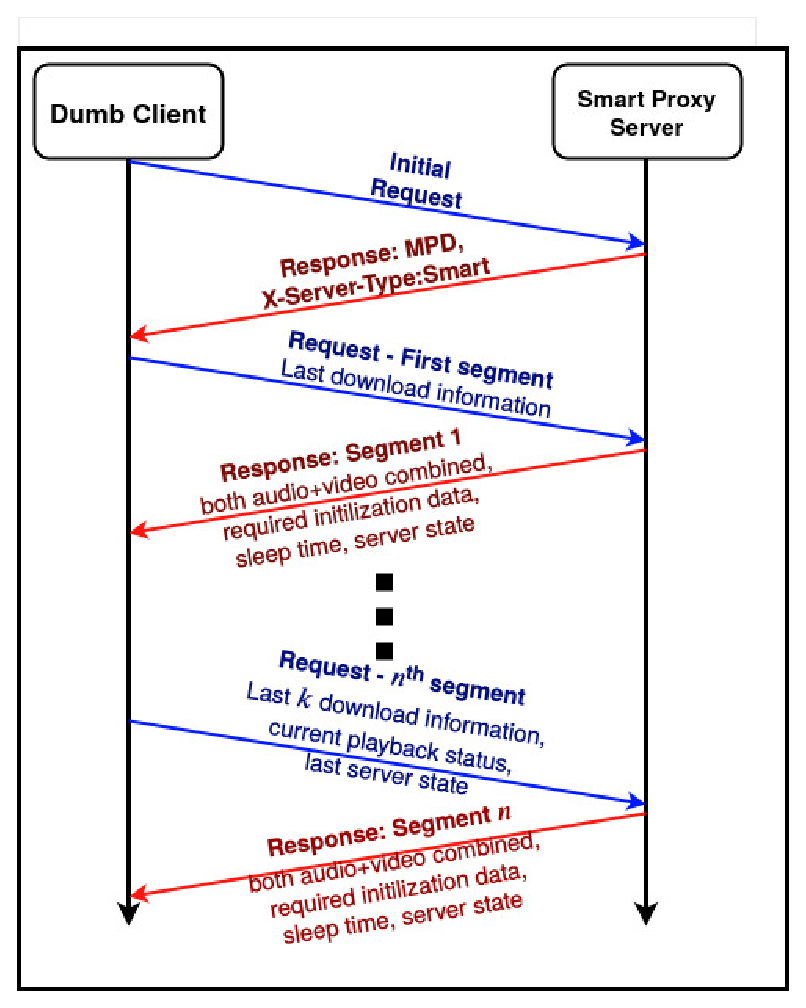
\includegraphics[width=0.5\linewidth]{img/splitDASHTransaction}
	\end{center}
	\caption{\label{fig:splitDASHTransaction} Modified DASH based streaming system to support ML based ABR algorithm}
\end{figure}

The Fig.~\ref{fig:splitDASHTransaction} depict the transaction between smart proxy server and dumb client. At first client request the Media Presentation Description (MPD) from the server. The smart proxy server returns a un-modified MPD for the video. However, it also adds a server identifier {\tt X-Server-Type: Smart}. This identifier indicate that the server is not simple CDN server, instead, it is a smart proxy server. So, the dumb client prepare the HTML video element and request for the first video segment. Here client does not mention the video/audio quality for the segment. Instead, client enclose the download history with the request. When the server receives a request, it looks for old server state in the request. If present, it will expand the state, other wise, it create a new state. Then, update the state according to the current playback information and download history provided in the request. Based on this information, server calculate the best quality for both audio and video segment based on the pre-decided ABR algorithm. Once quality is decided, it download the required segments of the calculated quality from the CDN/streaming (if not available in it cache) and send it back to the dumb player. It Also calculate the time player should wait (i.e. sleep time) before sending another request to the server. It multiplexes the sleep time and server state with the request. The contents of the server state is dependent of the ABR algorithm. Most of the deterministic ABR algorithm, does not required to maintain any state, however, ABR algorithm like pensieve need to maintain state. In case of pensieve, server state contains only the pensieve state.
Here we send the server state to client to make server stateless. The client does not read the server state, however, it store it and send with next request. As the server server state contain all the information regarding the server, client can send same request multiple time, and with server responses with same action for all of them. This very important as a response might get lost and client might need to resend the request to the server.

\noteam{need to add overhead with a table or plot}
